% !TeX root=main.tex

\section{Validation}
\label{sec:validation}
To verify the accuracy of the analytical model it has been validated using a discrete event simulator built in OMNeT++ \cite{VargaH08}. Each simulation experiment was run until the network reaches its steady state where further network cycles do not change the collected statistics appreciably.

Numerous validation experiments were performed for several combinations of network sizes, service lengths, number and probability of selection, and $p_{sdn\_root}$. To remain concise latency results are presented for selected cases. For all cases, where not otherwise specified, the following parameter settings are used:

\begin{itemize}
\item $k = 4$, $k_{vsw} = 2$ and $p_{sdn\_root} = 0$
\item All switches and the root SDN controller have the same service rate of 40 messages per cycle ($\mu = 40$, $\mu_{sdn} = 40$)
\item The VNFs have a service rate of 20 messages per cycle ($\mu_{vnf} = 20$)
\item The network holds one service with two VNFs
\item Services are selected with equal probability
\end{itemize}

% Different Number of Ports
\begin{figure*}[bt]
\centering
\begin{minipage}[b]{.48\textwidth}
	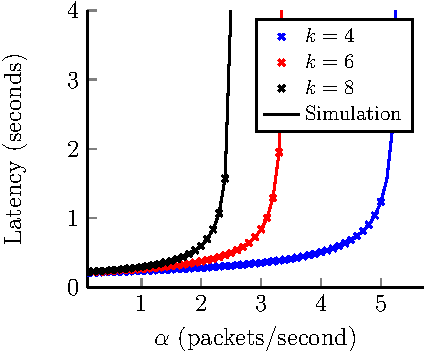
\includegraphics[width=\linewidth]{graphs/num_ports-crop}
	\caption{Latency predicted by the model and simulation for different numbers
of ports ($k$).} 
	\label{fig:num_ports}
\end{minipage}
\hfill
\begin{minipage}[b]{.48\textwidth}
	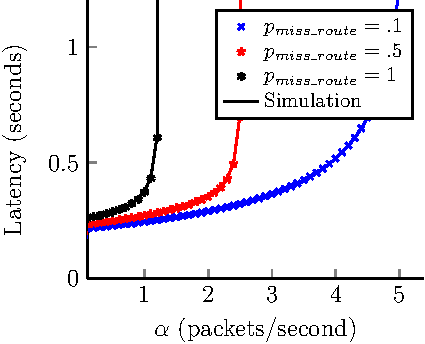
\includegraphics[width=\linewidth]{graphs/diff_sdn-crop}
	\caption{Latency predicted by the model and simulation with different
proportions of packets routing via the SDN controller ($p_{sdn\_root}$).}
	\label{fig:sdn_perc}
\end{minipage}

\vspace{10mm}

\begin{minipage}[b]{.48\textwidth}
	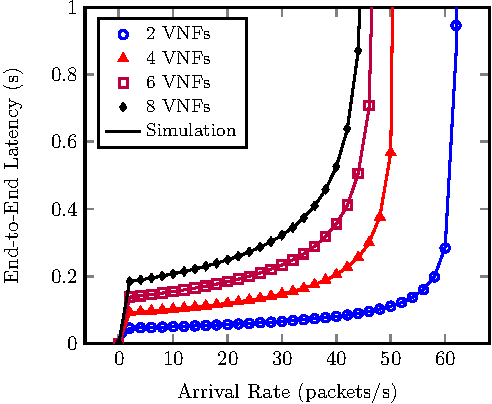
\includegraphics[width=\linewidth]{graphs/diff_lengths-crop}
	\caption{Latency predicted by the model and simulation for different length
service chains.}
	\label{fig:length_chain}
\end{minipage}
\hfill
\begin{minipage}[b]{.48\textwidth}
	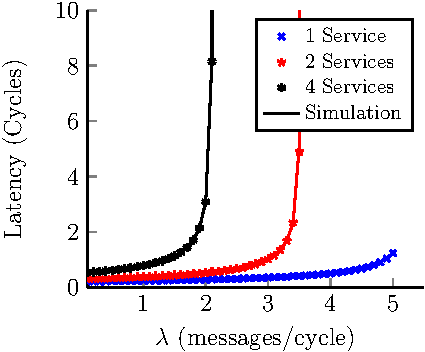
\includegraphics[width=\linewidth]{graphs/mult_services-crop}
	\caption{Latency predicted by the model and simulation for several services
of different lengths.}
	\label{fig:mult_services}
\end{minipage}

\end{figure*}

Additionally, when multiple services in the same network are considered (as in Figure \ref{fig:mult_services}) each service is assigned a length the same as its index plus one. As a consequence, tests with more services have higher average lengths. This decision was made to ensure the different tests were distinct from each other.

Figures \ref{fig:num_ports} to \ref{fig:mult_services} depict mean message latency predicted by the model plotted against those provided by a discrete event simulator for a range of parameter settings. For the model, results are only shown where the network is in a steady state, i.e. where the arrival rate for any network element is lower or equal to the service rate at the element. The figures demonstrate that the simulation results closely match those predicted by the model. The tractability and accuracy of the analytical model make it suitable for analysis of next generation NFV and SDN enabled communications networks.